% First LaTeX draft of the time-aware fusion paper (from the shared draft doc, 2026-10-17).
% Layout: IEEE two-column conference format on A4, as a page-count proxy for an ICRA
% workshop and for the two-column JSAI template. Swap the class once the venue is fixed.
\documentclass[conference,a4paper]{IEEEtran}

\usepackage[T1]{fontenc}
\usepackage{amsmath,amssymb}
\usepackage{booktabs}
\usepackage{xcolor}
\usepackage{tikz}
\usetikzlibrary{arrows.meta,positioning}
\usepackage{cite}
\usepackage[hidelinks]{hyperref}

\newcommand{\pending}[1]{\textcolor{red}{[PENDING: #1]}}
\newcommand{\todo}[1]{\textcolor{orange}{[TODO: #1]}}

\begin{document}

\title{Time Is the Baseline to Beat: Calibrated Fusion of\\
Policy-Internal Scores and Elapsed Time for VLA Failure Detection}

\author{\IEEEauthorblockN{Felix Doublet}
\IEEEauthorblockA{Shinoda Lab \todo{affiliation and co-authors}}}

\maketitle
\thispagestyle{plain}
\pagestyle{plain}

\begin{abstract}
Runtime failure detectors for vision-language-action (VLA) policies are rarely compared
against a simple competitor: elapsed time. Failed rollouts tend to run until the task
timeout, so a task-conditioned time-risk detector that sees no policy features already
catches 63\% of failures at a 5\% false-positive rate (FPR) on 38 RoboCasa365 tasks with
Xiaomi-Robotics-1. We study how policy-internal failure scores should be combined with
elapsed time under a frozen protocol at a matched FPR, with disjoint development,
calibration and prospective test cohorts. A preregistered design that let SAFE alarm only
in the first quarter of a rollout raised recall only from 0.632 to 0.668. Simple
time-aware fusion---alarm when either the policy-internal score or the time risk crosses
its threshold, with both thresholds calibrated jointly---reached 0.955 recall at 0.058 FPR
on 760 prospective rollouts. Four success-only anomaly scores fused the same way reached
0.905--0.947, statistically indistinguishable from fused SAFE. The gain therefore comes
from fusing a policy-internal signal with elapsed time, not from a particular learned
score. No detector gives early warning: at most 3\% of failures are caught by a quarter of
the task horizon. \pending{one sentence on the confirmatory test.}
\end{abstract}

\section{Introduction}

A failure detector earns its place only if it beats what a robot already knows for free:
how long the current attempt has been running. Generalist VLA policies still fail often on
household tasks, and a deployed system needs an online signal that a rollout is going
wrong. Recent detectors read the policy's internal features and learn to predict eventual
failure~\cite{gu2025safe}. Others score how unusual those features are relative to
successful rollouts~\cite{xu2025faildetect,lee2018mahalanobis,sun2022knn}.

These detectors are usually evaluated on completed rollouts, where a strong shortcut hides.
Successful rollouts stop at first success, while failures typically run to the timeout. In
our data, completed-rollout duration alone reaches ROC-AUC 0.80, more than the raw SAFE
score. A causal version of this shortcut is legitimate at deployment: the probability that
the task will fail, given that it is still running at step $t$. Any learned detector must
therefore beat this elapsed-time risk at the same false-positive budget, not just chance.

We make this comparison under a strict protocol. Detectors are developed on one cohort,
their thresholds are frozen on a separate calibration cohort at a 5\% event-level FPR, and
they are then evaluated once on a disjoint prospective cohort. We write down how each
outcome will be interpreted before opening each new result. Our contributions are:
\begin{enumerate}
  \item \textbf{Elapsed time as the reference.} A task-conditioned time-risk detector
  catches 63.2\% of failures at 4.7\% FPR on 760 prospective rollouts of
  Xiaomi-Robotics-1 on 38 RoboCasa365 tasks. Policy-feature scores used alone do worse at
  the same budget.
  \item \textbf{Time-aware fusion.} Alarming when either a policy-internal score or the
  time risk crosses a jointly calibrated threshold raises recall to 95.5\% at 5.8\% FPR,
  and also alarms earlier on average once missed failures are counted.
  \item \textbf{The representation matters less than the fusion.} SAFE, Mahalanobis, kNN,
  PCA-KMeans and RND scores all reach 90--95\% recall once fused with time, within
  confidence interval of each other. Success-only scores need no failure labels.
  \item \textbf{What did not work, reported as preregistered.} Restricting the policy
  score to the first quarter of the rollout, our original design, gained only 3.7 points
  of recall over time alone. No detector gives early warning by a quarter of the horizon.
\end{enumerate}
\pending{contribution 5, the result of the confirmatory test on a fresh cohort.}

\section{Related Work}

\textbf{Failure detection from policy internals.} SAFE trains a small MLP or LSTM on a
VLA's internal features to predict eventual failure, and thresholds it with functional
conformal prediction~\cite{gu2025safe}; we reuse its implementation. SAFE also notes that a
detector could simply count elapsed time, and removes this shortcut by truncating rollouts to
equal length when computing ROC-AUC. We keep elapsed time instead, as a deployable baseline
and a signal to fuse. Recent probes improve labels, robustness or
calibration~\cite{park2026hideseek,ma2026failurespot,rajaprakash2026safecast}, and VLA-Scope
adds execution-progress features to a learned predictor~\cite{zhu2026vlascope}. None compares
against elapsed time alone.

\textbf{Detectors without failure data.} FAIL-Detect scores policy inputs and outputs
against successful rollouts only~\cite{xu2025faildetect}. FIPER alarms when an RND score on
policy embeddings and an action-chunk entropy \emph{both} exceed conformal
thresholds~\cite{romer2025fiper}. Our success-only baselines follow the same idea, but our
fusion fires when \emph{either} of two signals crosses, so that each can catch failures the
other misses.

\textbf{Consistency and VLM monitors.} STAC~\cite{agia2024sentinel},
VLA-FAIL~\cite{seligmann2026vlafail} and ActProbe~\cite{huang2026actprobe} compare the
overlapping parts of consecutive action chunks. Xiaomi-Robotics-1 executes each 16-step chunk
in full, so this signal is undefined for our policy. VLM monitors judge task progress or
explain failures from frames~\cite{agia2024sentinel,duan2025aha} and are complementary to the
time signal.

\textbf{OOD scores and calibration.} We use SAFE's embedding baselines: Mahalanobis
distance~\cite{lee2018mahalanobis}, $k$-nearest-neighbour distance~\cite{sun2022knn}, PCA
plus $k$-means distance, and random network distillation~\cite{burda2019rnd}, all fitted on
successful rollouts. Conformal thresholds give finite-sample false-positive control under
exchangeability~\cite{angelopoulos2021gentle}. Most prior evaluations report ROC-AUC and one
operating point on the test pool. We instead freeze every threshold on a separate calibration
cohort and compare detectors at a matched event-level FPR on a disjoint prospective cohort.

\section{Problem Setting and Metrics}

A detector watches one rollout of a known task $k$ and decides online, at each genuine
policy inference $t$, whether to raise an alarm. Its score at $t$ may use only what is
available by $t$: the policy features so far, the inference index and the task identity.
It may not use the rollout's final length, future features, or subtask annotations. The
first threshold crossing is the alarm; the detector never changes the policy's actions.

Failure is the positive class. A failed rollout is detected if any alarm fires before it
ends; a successful rollout with any alarm is a false positive. We report event-level TPR
and FPR, balanced accuracy (BA), the \emph{miss-adjusted detection fraction}---the
first-alarm time as a fraction of the task horizon $H_k$, averaged over all failures with a
missed failure counted as 1.0 (lower is earlier)---and recall at 10\%, 25\% and 50\% of
$H_k$. All detectors are compared at operating points fixed on the calibration cohort under
FPR $\le 0.05$. Confidence intervals come from a paired bootstrap that resamples tasks, then
rollouts within each task (2,000 replicates).

\section{Method}

\begin{figure}[t]
\centering
\resizebox{\columnwidth}{!}{%
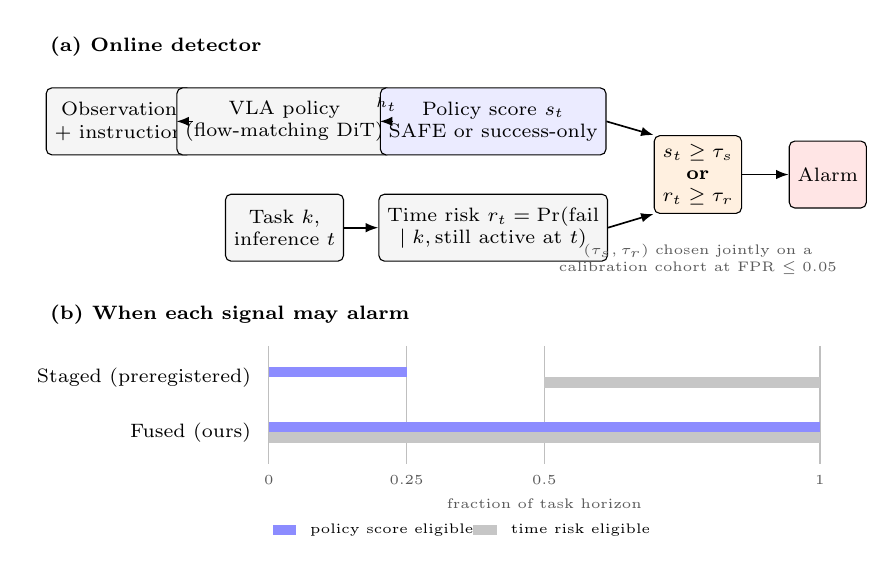
\begin{tikzpicture}[font=\scriptsize,
  box/.style={draw, rounded corners=2pt, align=center, minimum height=0.85cm, inner sep=3pt},
  arr/.style={-{Latex[length=1.6mm]}, semithick}]
  % (a) pipeline
  \node[anchor=west,font=\scriptsize\bfseries] at (-1.0,0.95) {(a) Online detector};
  \node[box, fill=gray!8] (obs) at (0,0) {Observation\\+ instruction};
  \node[box, fill=gray!8] (vla) at (2.1,0) {VLA policy\\(flow-matching DiT)};
  \node[box, fill=blue!8] (score) at (4.75,0) {Policy score $s_t$\\SAFE or success-only};
  \node[box, fill=gray!8] (task) at (2.1,-1.35) {Task $k$,\\inference $t$};
  \node[box, fill=gray!8] (time) at (4.75,-1.35) {Time risk $r_t = \Pr(\text{fail}$\\$\mid k, \text{still active at } t)$};
  \node[box, fill=orange!12] (or) at (7.35,-0.675) {$s_t \ge \tau_s$\\\textbf{or}\\$r_t \ge \tau_r$};
  \node[box, fill=red!10] (alarm) at (9.0,-0.675) {Alarm};
  \draw[arr] (obs) -- (vla);
  \draw[arr] (vla) -- node[above, font=\tiny] {$h_t$} (score);
  \draw[arr] (task) -- (time);
  \draw[arr] (score.east) -- (or.north west);
  \draw[arr] (time.east) -- (or.south west);
  \draw[arr] (or) -- (alarm);
  \node[align=center, font=\tiny, text=gray!70!black] at (7.35,-1.75)
    {$(\tau_s,\tau_r)$ chosen jointly on a\\calibration cohort at FPR $\le 0.05$};
  % (b) eligibility windows
  \node[anchor=west,font=\scriptsize\bfseries] at (-1.0,-2.45) {(b) When each signal may alarm};
  \def\xa{1.9} \def\xb{8.9}
  \foreach \f/\l in {0/0, 0.25/0.25, 0.5/0.5, 1/1}{
    \draw[gray!50] ({\xa+\f*(\xb-\xa)},-2.85) -- ({\xa+\f*(\xb-\xa)},-4.35);
    \node[gray!70!black, font=\tiny] at ({\xa+\f*(\xb-\xa)},-4.55) {\l};
  }
  \node[gray!70!black, font=\tiny] at ({(\xa+\xb)/2},-4.85) {fraction of task horizon};
  \node[anchor=east] at (\xa-0.1,-3.25) {Staged (preregistered)};
  \fill[blue!45] (\xa,-3.12) rectangle ({\xa+0.25*(\xb-\xa)},-3.25);
  \fill[gray!45] ({\xa+0.5*(\xb-\xa)},-3.25) rectangle (\xb,-3.38);
  \node[anchor=east] at (\xa-0.1,-3.95) {Fused (ours)};
  \fill[blue!45] (\xa,-3.82) rectangle (\xb,-3.95);
  \fill[gray!45] (\xa,-3.95) rectangle (\xb,-4.08);
  \fill[blue!45] (\xa+0.05,-5.25) rectangle (\xa+0.35,-5.12);
  \node[anchor=west, font=\tiny] at (\xa+0.4,-5.185) {policy score eligible};
  \fill[gray!45] (\xa+2.6,-5.25) rectangle (\xa+2.9,-5.12);
  \node[anchor=west, font=\tiny] at (\xa+2.95,-5.185) {time risk eligible};
\end{tikzpicture}}
\caption{Time-aware fusion. (a) At each policy inference, a policy-internal score and a
task-conditioned elapsed-time risk are compared with two thresholds; the first crossing of
either raises the alarm. Both thresholds are set together on a separate calibration cohort.
(b) The preregistered staged design let the policy score alarm only in the first quarter of
the rollout and time only after half; fusion lets both alarm throughout.}
\label{fig:method}
\end{figure}

Time-aware fusion (Fig.~\ref{fig:method}) combines two causal scores, each with its own
threshold, and alarms as soon as either crosses. Both thresholds are chosen together on a calibration cohort so that
the combined detector meets the FPR budget.

\subsection{Policy-internal score}

\textbf{SAFE.} At each inference we take the final-layer action-token hidden state of the
policy's flow-matching DiT, just before its action output layer (1,024 dimensions, last
flow step, last action position). The official SAFE MLP maps it to a failure score. We
standardize scores per task using statistics from training rollouts only, take the running
maximum over the rollout, and average three seeds to obtain $s_t$.

\textbf{Success-only scores.} Mahalanobis, cosine kNN, PCA-KMeans and feature-space RND
are fitted on successful development rollouts only, so they need no failure labels. Each
produces a per-inference distance, aggregated causally (development selected a cumulative
sum for all four) and normalized per task. Hyperparameters were chosen on held-out
development data by early at-risk ROC-AUC.

\subsection{Elapsed-time risk}

The time risk is the probability that a still-running rollout of task $k$ will fail,
estimated from training rollouts as a monotone curve per task:
\begin{equation}
  r_t = \Pr(\text{failure} \mid \text{task } k,\ \text{rollout still active at inference } t).
\end{equation}
It needs no policy features and is causal, because it uses only whether the rollout is
still running.

\subsection{Calibrated fusion}

The fused detector alarms at the first inference where either score crosses its threshold:
\begin{equation}
  T_{\text{alarm}} = \min \{\, t : s_t \ge \tau_s \ \text{or}\ r_t \ge \tau_r \,\}.
\end{equation}
The pair $(\tau_s, \tau_r)$ is searched jointly on the calibration cohort. Among pairs with
event-level FPR $\le 0.05$, we keep the one with the highest recall, then the earliest
miss-adjusted detection, then the more conservative thresholds. A successful rollout counts
as a false positive if either score alarms at any time.

\subsection{Staged variant (preregistered)}

Our original design restricted the policy score to the start of the rollout, where elapsed
time cannot separate outcomes, and used time as a late fallback: the policy score may alarm
only while $t \le 0.25 H_k$, and the time risk only from $t \ge 0.5 H_k$. Thresholds are
searched the same way. We froze this variant before the prospective test and report it as
preregistered.

\section{Experimental Setup}

\begin{table*}[t]
\centering
\caption{Paired differences on the prospective test (task-then-rollout bootstrap, 95\% CI).
BA = balanced accuracy; adj = miss-adjusted detection fraction (lower is earlier).}
\label{tab:main}
\footnotesize
\begin{tabular}{@{}lcccc@{}}
\toprule
Detector & BA & adj & $\Delta$ recall vs.\ time only & $\Delta$ recall vs.\ fused SAFE + time \\
\midrule
Time only & 0.792 & 0.880 & -- & $-0.324$ [$-0.469$, $-0.178$] \\
SAFE only & 0.763 & 0.810 & $-0.065$ [$-0.354$, $+0.215$] & $-0.389$ [$-0.568$, $-0.218$] \\
Staged SAFE + time (preregistered) & 0.809 & 0.854 & $+0.037$ [$+0.000$, $+0.090$] & $-0.287$ [$-0.426$, $-0.156$] \\
Staged kNN + time & 0.803 & 0.857 & $+0.035$ [$+0.000$, $+0.097$] & $-0.289$ [$-0.431$, $-0.157$] \\
\midrule
\textbf{Fused SAFE + time} & \textbf{0.949} & 0.816 & $\mathbf{+0.324}$ [$+0.178$, $+0.469$] & -- \\
Fused kNN + time & 0.939 & \textbf{0.769} & $+0.316$ [$+0.142$, $+0.495$] & $-0.008$ [$-0.093$, $+0.072$] \\
Fused Mahalanobis + time & 0.936 & 0.783 & $+0.308$ [$+0.133$, $+0.484$] & $-0.016$ [$-0.097$, $+0.065$] \\
Fused PCA-KMeans + time & 0.932 & 0.785 & $+0.293$ [$+0.105$, $+0.479$] & $-0.031$ [$-0.130$, $+0.061$] \\
Fused RND + time & 0.921 & 0.794 & $+0.275$ [$+0.082$, $+0.469$] & $-0.049$ [$-0.153$, $+0.050$] \\
\bottomrule
\end{tabular}
\end{table*}


\textbf{Policy and tasks.} We use the released Xiaomi-Robotics-1 RoboCasa365
checkpoint~\cite{xiaomi2026robotics} at a pinned revision. It predicts 16-step action chunks
with a five-step flow-matching DiT and executes each chunk in full. We take the 39 official
RoboCasa365 tasks~\cite{nasiriany2024robocasa,robocasa365} whose published success count
lies between 5 and 45 out of 50, and drop one with too few failures, leaving 38 tasks
(10 atomic, 28 composite).



\textbf{Cohorts.} We use four disjoint cohorts, each for one purpose: 1,824 development rollouts train SAFE and fit the scores and time curves; 228 calibration rollouts (114 per class, 454 retained) choose every threshold; 760 prospective test rollouts (380 per class, 1,643 retained) give one evaluation of the frozen detectors; and a 760-rollout confirmatory cohort \pending{in collection}. Calibration and test cohorts take the first 3 or 10 successes and failures per task from fresh environment seeds, keep every overshoot rollout as a secondary cohort, and never share seeds.

\textbf{Frozen protocol.} The staged detector, all SAFE checkpoints, normalization and time
curves were frozen before the prospective test was collected. The baselines and fused
detectors were added later and evaluated once on the same opened cohort, with thresholds
taken from calibration only. Each run first had to reproduce the frozen results and
thresholds exactly and verify the checksums of the frozen inputs. Before each new
evaluation we wrote down how we would interpret every outcome, including the rule for
crediting SAFE specifically.

\textbf{Detectors compared.} Time only; SAFE only; staged SAFE + time (preregistered); fused
SAFE + time; and each success-only score alone, staged with time, and fused with time.

\section{Results}

On the 760-rollout prospective test, every policy-internal score fused with elapsed time
detects 90--96\% of failures at about 6\% FPR, against 63\% for time alone
(Fig.~\ref{fig:points}, Table~\ref{tab:main}).

\begin{figure}[t]
\centering
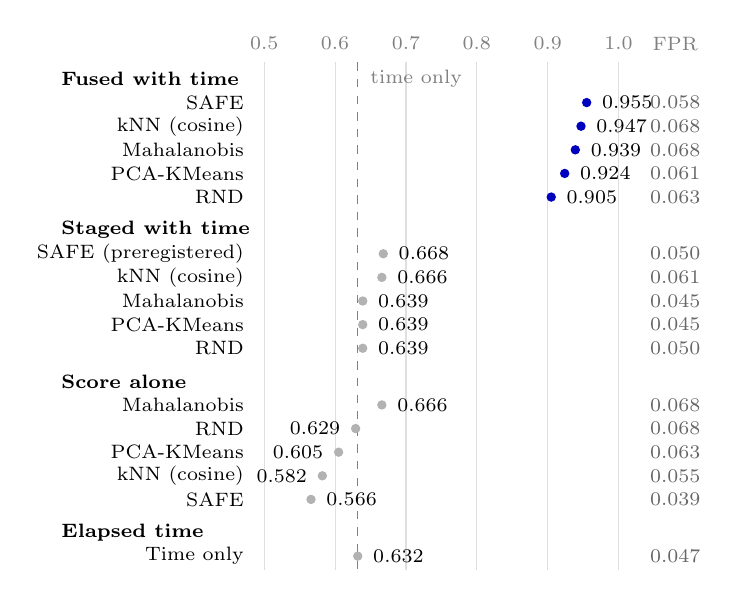
\begin{tikzpicture}[x=9cm,y=0.3cm,font=\scriptsize]
  % grid and tick labels (recall 0.5 to 1.0)
  \foreach \t in {0.5,0.6,0.7,0.8,0.9,1.0}{
    \draw[gray!25] ({\t-0.5},0.7) -- ({\t-0.5},-20.8);
    \node[gray] at ({\t-0.5},1.5) {\t};
  }
  \node[gray] at (0.58,1.5) {FPR};
  % time-only reference
  \draw[dashed,gray] ({0.632-0.5},0.7) -- ({0.632-0.5},-20.8);
  \node[gray,anchor=west] at ({0.632-0.5+0.004},0) {time only};
  % family headers
  \foreach \y/\h in {0/Fused with time,-6.4/Staged with time,-12.8/Score alone,-19.2/Elapsed time}{
    \node[anchor=west,font=\scriptsize\bfseries] at (-0.30,\y) {\h};
  }
  % rows: y / name / recall / test FPR / colour / label anchor / label offset
  \foreach \y/\n/\r/\f/\c/\a/\o in {
      -1/SAFE/0.955/0.058/blue!75!black/west/0.008,
      -2/kNN (cosine)/0.947/0.068/blue!75!black/west/0.008,
      -3/Mahalanobis/0.939/0.068/blue!75!black/west/0.008,
      -4/PCA-KMeans/0.924/0.061/blue!75!black/west/0.008,
      -5/RND/0.905/0.063/blue!75!black/west/0.008,
      -7.4/SAFE (preregistered)/0.668/0.050/gray!60/west/0.008,
      -8.4/kNN (cosine)/0.666/0.061/gray!60/west/0.008,
      -9.4/Mahalanobis/0.639/0.045/gray!60/west/0.008,
      -10.4/PCA-KMeans/0.639/0.045/gray!60/west/0.008,
      -11.4/RND/0.639/0.050/gray!60/west/0.008,
      -13.8/Mahalanobis/0.666/0.068/gray!60/west/0.008,
      -14.8/RND/0.629/0.068/gray!60/east/-0.008,
      -15.8/PCA-KMeans/0.605/0.063/gray!60/east/-0.008,
      -16.8/kNN (cosine)/0.582/0.055/gray!60/east/-0.008,
      -17.8/SAFE/0.566/0.039/gray!60/west/0.008,
      -20.2/Time only/0.632/0.047/gray!60/west/0.008}{
    \node[anchor=east] at (-0.015,\y) {\n};
    \fill[\c] ({\r-0.5},\y) circle (1.7pt);
    \node[anchor=\a] at ({\r-0.5+\o},\y) {\r};
    \node[gray!80!black] at (0.58,\y) {\f};
  }
\end{tikzpicture}
\caption{Recall of every detector on the prospective test (380 failures), with thresholds
frozen on calibration at FPR $\le 0.05$; observed test FPR at right. All fused detectors
sit near 0.90--0.96 recall, while staged and standalone detectors stay near time only.}
\label{fig:points}
\end{figure}

\begin{table}[t]
\centering
\caption{Recall / FPR by task type on the prospective test (atomic: 10 tasks, 100 rollouts
per class; composite: 28 tasks, 280 per class). Descriptive only.}
\label{tab:strata}
\footnotesize
\begin{tabular}{@{}lcc@{}}
\toprule
Detector & Atomic & Composite \\
\midrule
Time only & 0.400 / 0.020 & 0.714 / 0.057 \\
SAFE only & 0.800 / 0.080 & 0.482 / 0.025 \\
Staged SAFE + time & 0.540 / 0.040 & 0.714 / 0.054 \\
Fused SAFE + time & 0.980 / 0.030 & 0.946 / 0.068 \\
Fused kNN + time & 0.940 / 0.080 & 0.950 / 0.064 \\
Fused Mahalanobis + time & 0.890 / 0.050 & 0.957 / 0.075 \\
\bottomrule
\end{tabular}
\end{table}



\subsection{Elapsed time is a strong reference}

Time only reaches 0.632 recall at 0.047 FPR without any policy feature. SAFE alone reaches
0.566 at 0.039. The success-only scores alone reach 0.58--0.67, but at FPRs of 0.055--0.068,
and their cumulative-sum aggregation grows with elapsed time, so part of their signal is
duration.

\subsection{Fusion beats staging}

Fused SAFE + time detects 109 more failures than the staged design (363 against 254 of 380)
for 3 more false alarms (22 against 19 of 380). It is also earlier once misses are counted:
miss-adjusted detection improves by 0.038 of the horizon (95\% CI 0.006--0.070). Most of the
policy score's complementary evidence arrives after the first quarter of the rollout, which
the staged design discards.

\subsection{The representation matters less than the fusion}

All four success-only scores fused with time come within confidence interval of fused SAFE;
the largest gap is 0.049 recall (RND). Before evaluating, we had declared that SAFE would be
credited only if every fused baseline's recall difference had a CI entirely below zero.
None did, so we attribute the gain to fusing a policy-internal score with elapsed time.
Fused SAFE keeps the lowest FPR among fused detectors (0.058 against 0.061--0.068), and fused
kNN alarms earliest (0.769), but neither difference is decisive. Inside the staged wrapper,
the baselines trail SAFE by 0.002--0.029 recall, with every CI reaching zero.

\subsection{Atomic and composite tasks}



Time alone is weak on atomic tasks and SAFE alone is weak on composites, and fusion repairs
both (Table~\ref{tab:strata}). On atomic tasks fused SAFE has the best recall/FPR trade-off;
on composites all fused scores are equivalent. We read this as consistent with a label
mismatch: a terminal outcome label fits one atomic attempt, but marks the correct early work
of a long composite task as failing.

\subsection{No early warning}

No detector catches more than 2.9\% of failures by 25\% of the task horizon; fused detectors
catch none. Fusion improves detection before the rollout ends, not early warning.

\subsection{Confirmatory test}

\pending{the preregistered test of fused SAFE + time against time only on 760 fresh rollouts
(base seed 1300007), with fused kNN + time as the declared secondary. Criteria: bootstrap CI
of the recall gain above zero, a point gain of at least 0.15, and test FPR at most 0.075
with Wilson upper bound at most 0.10.}

\section{Discussion and Limitations}

The practical lesson is to evaluate any learned failure detector against a calibrated
elapsed-time detector, and to deploy it fused with one. We hypothesize that the two signals
catch different failures \todo{check per task}: time catches failures in tasks whose
successes finish quickly, while the policy score catches failures in tasks where successful
and failed rollouts run equally long. Because simple success-only scores work nearly as well
as SAFE once fused, a deployment can skip collecting labelled failures.

\textbf{Limitations.} (i)~The fused detectors were defined after the prospective cohort had
been opened for the staged design; their thresholds came only from calibration and each was
evaluated once, but only the confirmatory test makes the headline claim preregistered.
(ii)~Every detector held 0.044 FPR on calibration, while fused detectors reached 0.058--0.068
on the test, with Wilson intervals that include 0.05; calibration had only 114 successful
rollouts. (iii)~Alarms come late in the rollout, which may leave little time to recover.
(iv)~All results use one policy in simulation; earlier experiments with $\pi_0$ and RLDX-1
showed the same atomic-versus-composite gap on smaller datasets. (v)~Task normalization and
the time curves assume the deployed task and its horizon are known. (vi)~Test cohorts are
balanced by quota, so recall and FPR are reported per class rather than at deployment
prevalence.

\section{Conclusion}

Elapsed time is the baseline a VLA failure detector must beat, and fusing it with a
policy-internal score is the simplest way to beat it. On 760 prospective rollouts across 38
RoboCasa365 tasks, calibrated fusion detected 95.5\% of failures at 5.8\% FPR, against 63.2\%
for time alone. Which policy score is fused matters little. Stage-aware supervision that gives
early, localized warnings on long-horizon tasks is the natural next step.
\pending{confirmatory result.}

\bibliographystyle{IEEEtran}
\bibliography{refs}

\end{document}
